\section{Experimental Setup}

\subsection{Simulation Overview}

\begin{frame}{Overview} % _____________________________________________
  \begin{center}
  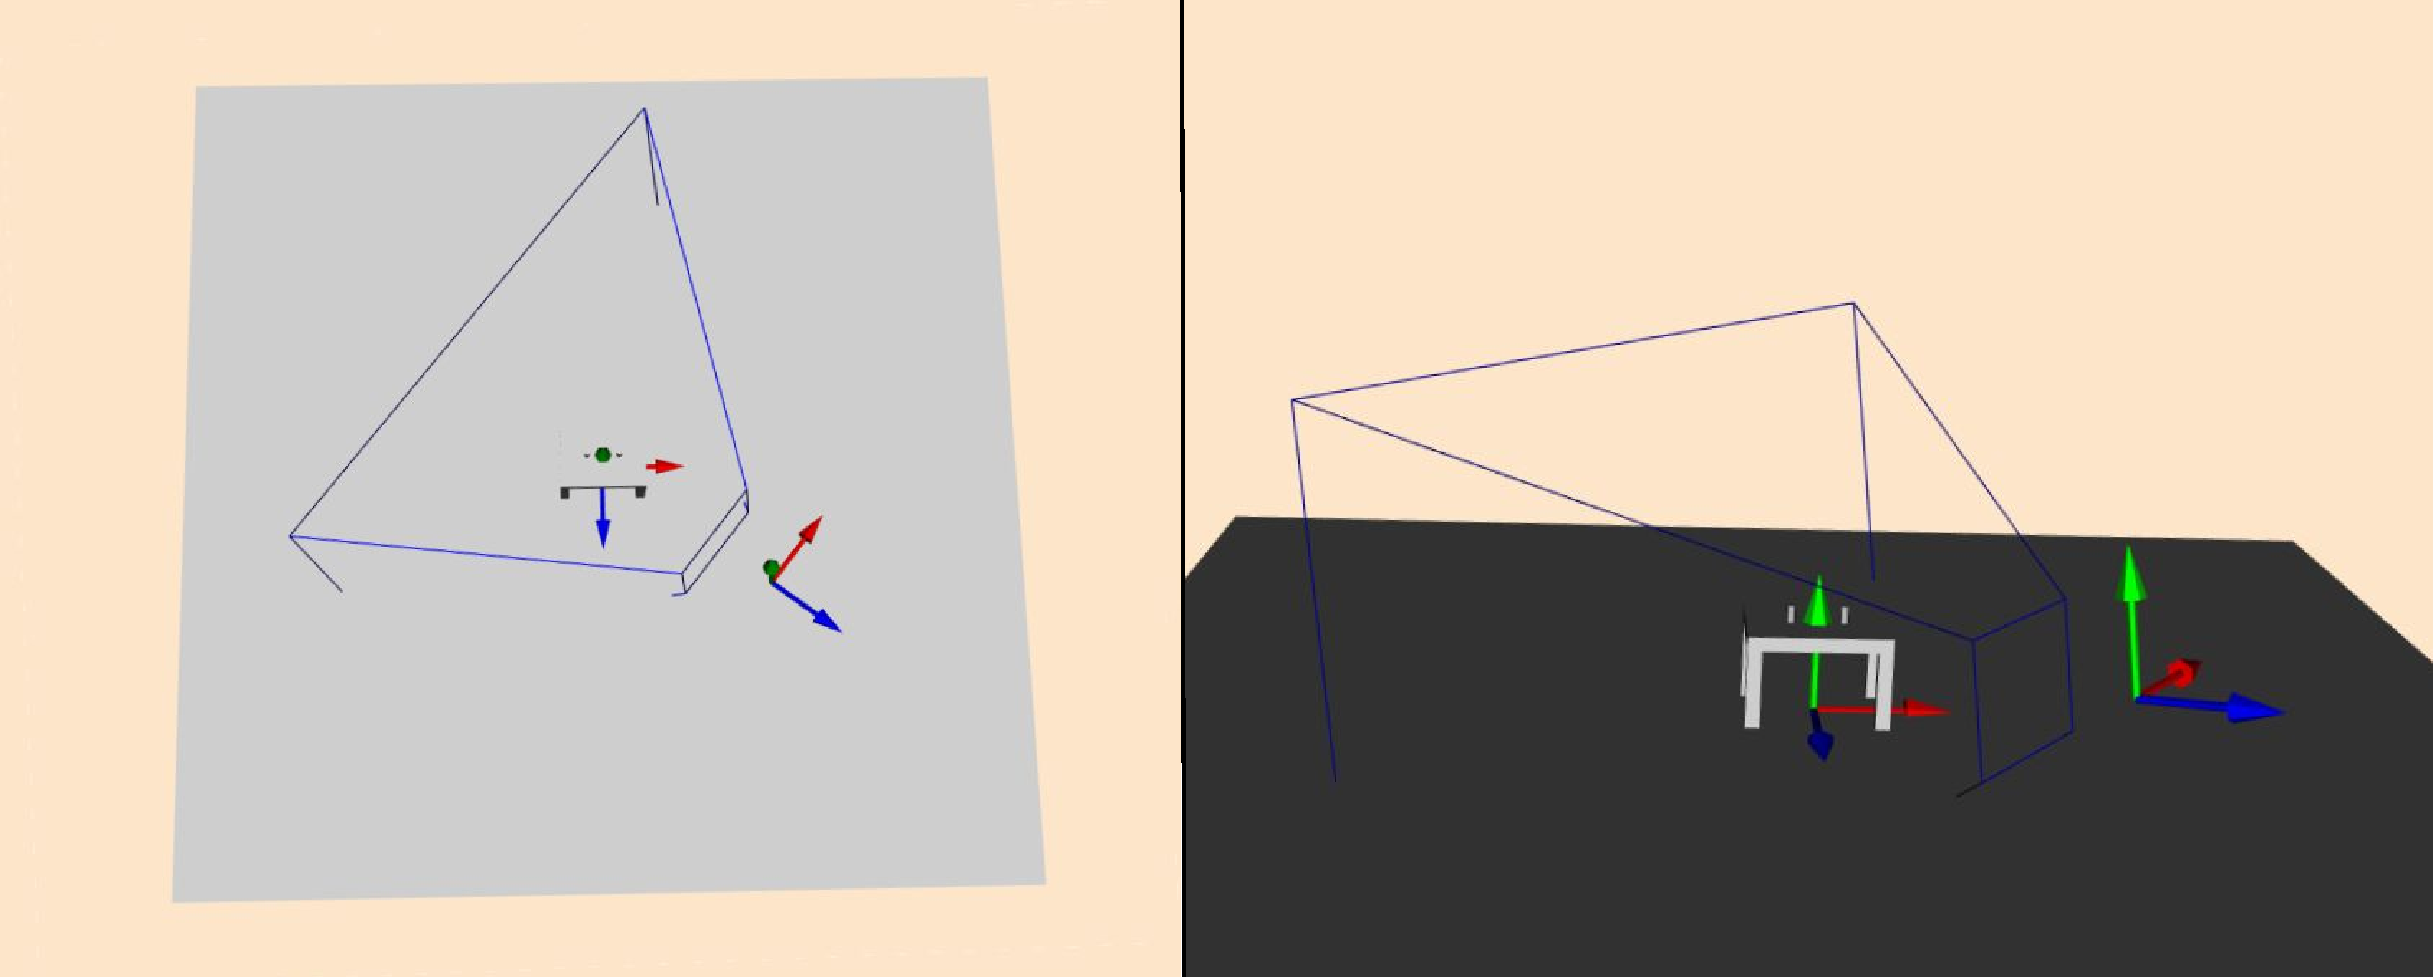
\includegraphics[width=\textwidth]
    {../figures/expsetup_simulation_overview.pdf}
  \end{center}
\end{frame}

\note[itemize]{
\item
}

\subsection{Simulating a RGB-D Sensor}

\begin{frame}{Rendering Pipeline} % ____________________________________________
  \begin{center}
  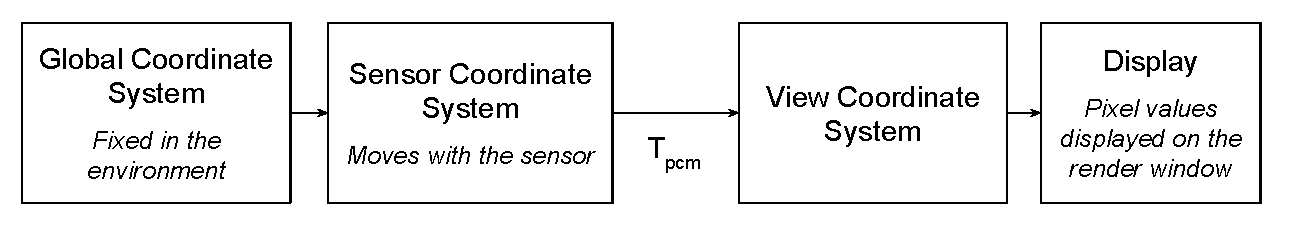
\includegraphics[width=\textwidth]
    {../figures/expsetup_render_pipeline.pdf}
  \end{center}
\end{frame}

\note[itemize]{
\item Render pipeline: projects 3D global coordinates to 2D pixel coordinates
}

\begin{frame}{$T_{pcm}$} % _____________________________________________________
  \vspace{-0.15in}
  \begin{center}
  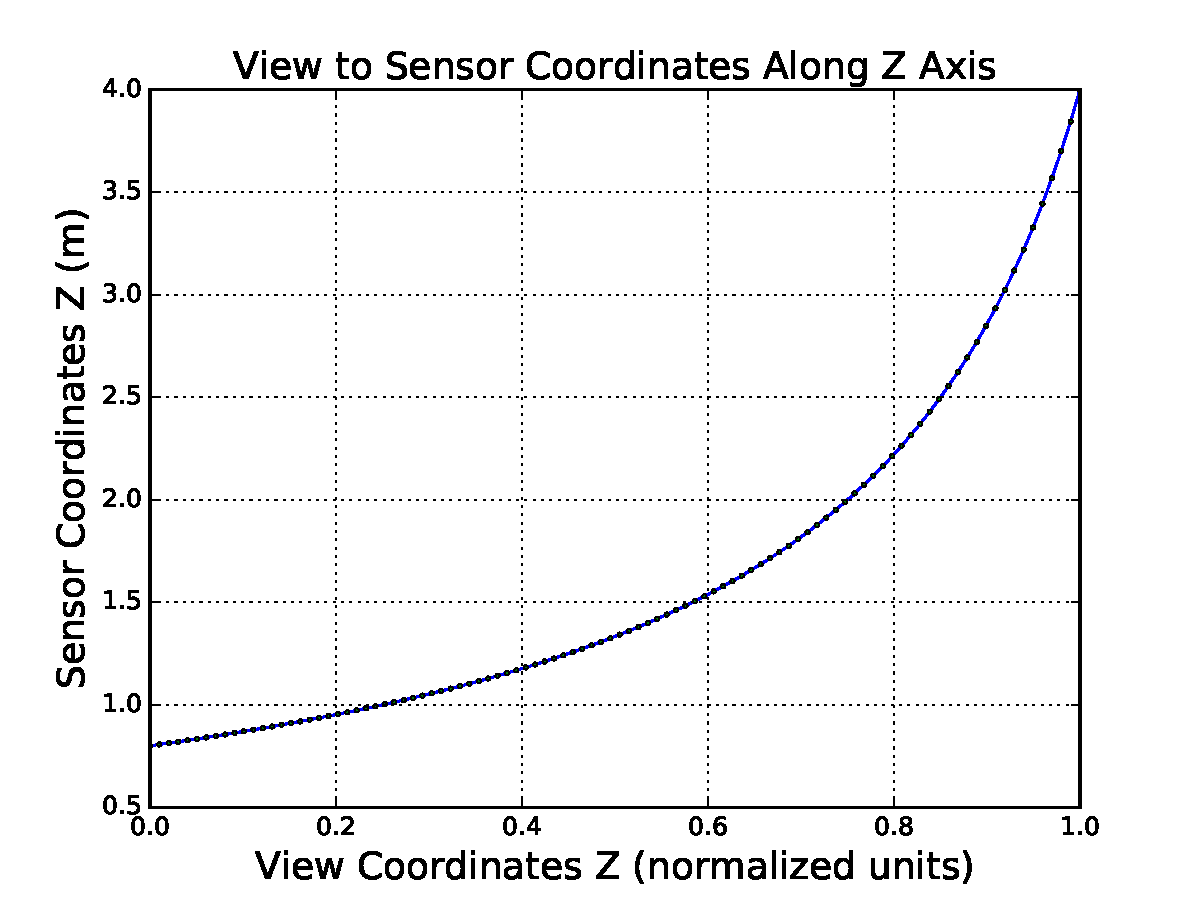
\includegraphics[height=0.90\textheight]
    {../figures/expsetup_depth_view_to_sensor.pdf}
  \end{center}
\end{frame}

\note[itemize]{
\item The pinhole camera transformation, $T_{pcm}$, creates a non-linear
relationship between values in the depth image and their corresponding location
in the sensor's coordinate system.
}

\begin{frame}{Adding Noise} % __________________________________________________
  \vspace{-0.15in}
  \begin{center}
  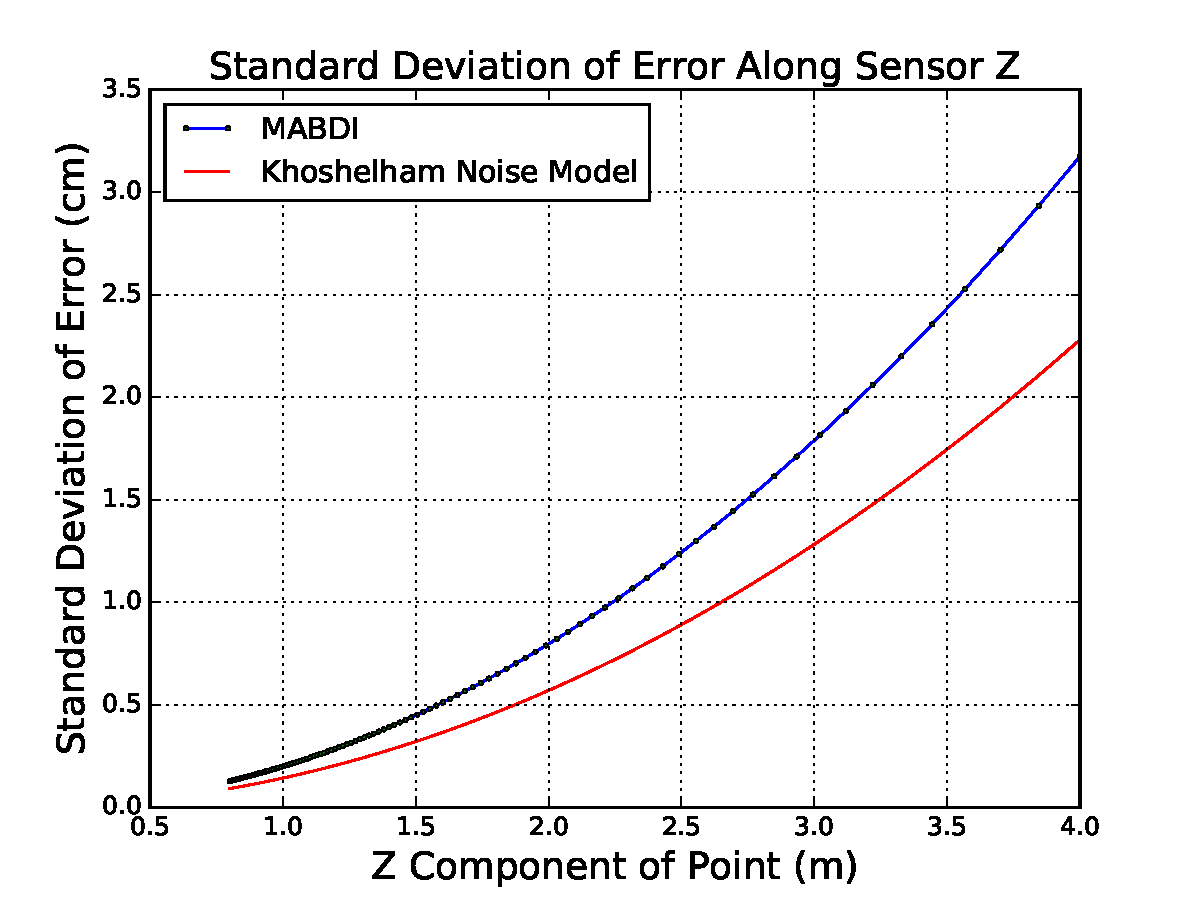
\includegraphics[height=0.90\textheight]
    {../figures/expsetup_noise_error.pdf}
  \end{center}
\end{frame}

\note[itemize]{
\item Comparison of standard deviation of the error used in the MABDI simulation and the error model from Khoshelham.
}

\subsection{Sensor Path}

\begin{frame}{Sensor Path} % __________________________________________________
  \vspace{-0.15in}
  \begin{center}
  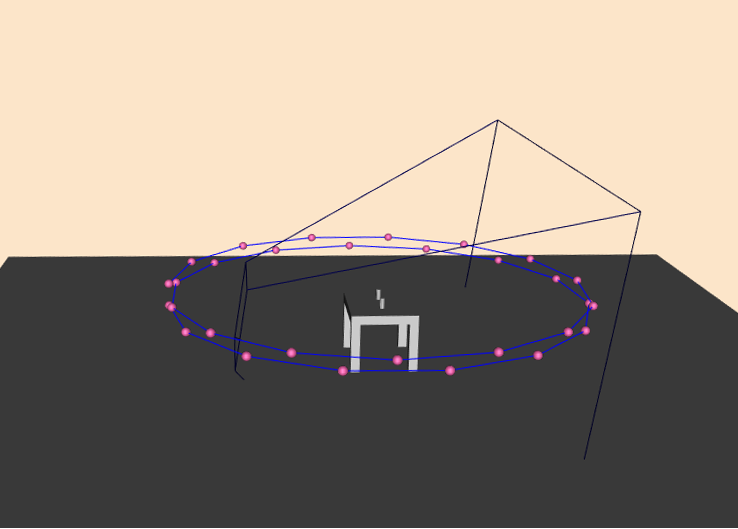
\includegraphics[height=0.90\textheight]
    {../figures/expsetup_path.png}
  \end{center}
\end{frame}

\note[itemize]{
\item The blue line indicates the path and the pink points indicate where the
sensor stops along the path. The path circles the objects in the environment
twice. A helical path was chosen because it returns to a part of the environment
that has already been mapped and is thus ``known'' to the algorithm. Also,
because the path is a helix and not just a circle, the sensor views the
environment from a slightly different position on each pass.
}

\subsection{Simulation Parameters}

\begin{frame}{Simulation Parameters} % _________________________________________
  \begin{table}[h]
    \begin{center}
      \begin{tabular}{|l|c|c|c|c|}
      \hline
             & Environment & Noise   & Dynamic & Iterations \\\hline
      Run 1	 & Table       & False   & False   & 30 \\
      Run 2  & Bunnies     & True    & False   & 50 \\
      Run 3  & Bunnies     & True    & True    & 50 \\
      \hline
      \end{tabular}
    \end{center}
  \end{table}
\end{frame}

\note[itemize]{
\item Environment - This parameter specifies the environment used to generate
the simulated depth images. \textit{Table} is an environment consisting of a
table and two cups placed on the table. The table is 1 meter tall.
\textit{Bunnies} is an environment consisting of three bunnies that are
around 1.5 meters tall. These bunnies are created using the Stanford Bunny a well known data set in computer graphics.
\item Noise - If true, adds noise to the depth image of the simulated sensor.
\item Dynamic - If true, adds an object during the simulation. In the case
of this analysis, a third bunny is added half-way through the simulation.
\item Iterations - The number of times MABDI will run. This number is equal to the number of stops the sensor makes along the path because every time the sensor stops MABDI is run to update the global mesh.
}
